\documentclass[xcolor={table}]{beamer}
\usepackage{fleqn}
\usepackage{graphicx}
\usepackage{coordsys} %for \numbline commander

%Setup appearance:
\usetheme{Darmstadt}
\usefonttheme[onlylarge]{structurebold}
\setbeamerfont*{frametitle}{size=\normalsize,series=\bfseries}
\setbeamertemplate{navigation symbols}{}
\setbeamertemplate{bibliography item}{[\theenumiv]}

% Standard packages
\usepackage[english]{babel}
\usepackage[latin1]{inputenc}
\usepackage{times}
\usepackage[T1]{fontenc}
\usepackage{multirow}
\usepackage{subfigure}
\usepackage{pbox}
\usepackage{arydshln}
\usepackage{pifont}
\usepackage{cancel}
\usepackage{rotating} % for sideways headings

% Source Code packages
\usepackage{algorithm2e}
\usepackage{algorithmic}

\DeclareSymbolFont{extraup}{U}{zavm}{m}{n}
\DeclareMathSymbol{\varclub}{\mathalpha}{extraup}{84}
\DeclareMathSymbol{\varspade}{\mathalpha}{extraup}{85}
\DeclareMathSymbol{\varheart}{\mathalpha}{extraup}{86}
\DeclareMathSymbol{\vardiamond}{\mathalpha}{extraup}{87}

%%% This section command that adds a big page with section dividers
\usepackage{xifthen}% provides \isempty test
\newcommand{\SectionSlide}[2][]{
	\ifthenelse{\isempty{#1}}
		{\section{#2}\begin{frame} \begin{center}\begin{huge}#2\end{huge}\end{center}\end{frame}}
		{\section[#1]{#2}\begin{frame} \begin{center}\begin{huge}#2\end{huge}\end{center}\end{frame}}
}
%Extends the section slide to to include a shortened section title for the navigation bar as a second parameter
\newcommand{\SectionSlideShortHeader}[3][]{
	\ifthenelse{\isempty{#1}}
		{\section[#3]{#2}\begin{frame} \begin{center}\begin{huge}#2\end{huge}\end{center}\end{frame}}
		{\section[#1]{#2}\begin{frame} \begin{center}\begin{huge}#3\end{huge}\end{center}\end{frame}}
}

\newcommand{\refer}[1]{\footnote{#1}}
\newcommand{\GW}{\text{\textit{Guess-Who~}}}
\newcommand{\keyword}[1]{\alert{\textbf{#1}}\index{#1}}
\newcommand{\firstkeyword}[1]{\textbf{#1}\index{#1}}
\newcommand{\indexkeyword}[1]{\alert{\textbf{#1}\index{#1}}}
\newcommand{\featN}[1]{\textsc{#1}}
\newcommand{\featL}[1]{\textit{'#1'}}
 \newcommand{\ourRef}[1]{\ref{#1} $^{\text{\tiny[\pageref{#1}]}}$}
 \newcommand{\ourEqRef}[1]{\eqref{#1}$^{\text{\tiny[\pageref{#1}]}}$}
  
\DeclareMathOperator*{\argmax}{argmax}
\DeclareMathOperator*{\argmin}{argmin}

\title{Appendix B Introduction to Probability\\for Machine Learning}
	\author{John D. Kelleher and Brian Mac Namee and Aoife D'Arcy}
	\institute{}
	\date{}

\begin{document}
\begin{frame}
	\titlepage
\end{frame}
\begin{frame}
	 \tableofcontents
\end{frame}

\section{Probability Basics}

 \begin{frame} 
 \begin{itemize}
	\item Probability is the branch of mathematics that deals with measuring the likelihood (or uncertainty) around events. 
	\item There are two ways of computing the likelihood  of a future event:
\begin{enumerate}
	\item use the \keyword{relative frequency} of the event in the past, 
	\item use a \keyword{subjective} estimate (ideally from an expert!)
\end{enumerate}
	\item We will focus on using relative frequency.
\end{itemize} 
\end{frame} 

 \begin{frame} 
\begin{figure}
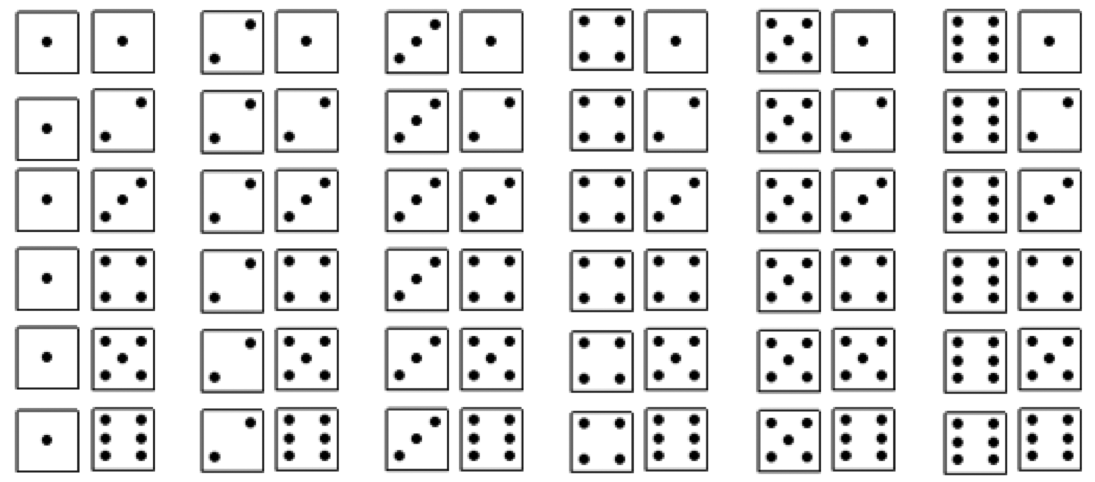
\includegraphics[width=\textwidth]{./images/samplespace2dice_BW_noBrackets.png}
\caption{The \keyword{sample space} for the domain of two dice.}
\label{fig:samplespacetwodice}
\end{figure}
\end{frame} 

 \begin{frame} 
\begin{table}
\centering
	\begin{footnotesize}
	\begin{tabular}{c c c}
	\hline
	\textbf{ID} & \textbf{Die1} & \textbf{Die2}\\
	\hline
		1 & 3 & 4\\
	      2 & 1 & 5\\
           3 & 6 & 5\\
           4 & 3 & 3\\
           5 & 1 & 1\\
	\hline
	\end{tabular}
	\end{footnotesize}
	\label{table:dicedataset}
	\caption{A dataset of instances from the sample space in Figure \ourRef{fig:samplespacetwodice}.}
\end{table}
\end{frame} 

 \begin{frame} 
\begin{itemize}
	\item Throughout our discussions about probability we will be talking about \keyword{events} so it is very important that you understand this simple concept.
\end{itemize}
\begin{alertblock}{Events}
\begin{itemize}
\item an \keyword{event} defines an assignment of values to the features in the domain; these assignments may define values for all the features in the domain (e.g. a full row in the dataset) or just to one or more features in the domain, 
\end{itemize}
\end{alertblock}
\begin{example}
\begin{itemize}
	\item \featN{Die1}=\featL{3}, 
	\item \featN{Die1}=\featL{1}, \featN{Die2}=\featL{5}.
\end{itemize}
\end{example}
\end{frame} 


 \begin{frame} 
\begin{alertblock}{Probability Functions: $P()$}
\begin{itemize}
	\item A feature can take one or more values from a domain and we can find out the likelihood of a feature taking any particular value using a \keyword{probability function} $P()$. 
	\item A probability function is a function that takes an event (an assignment of values to features) as a parameter and returns the likelihood of that event. 
	\end{itemize}
\end{alertblock}
	\begin{example}
		\begin{itemize}
			\item $P(\featN{Die1}=\featL{3})$ will return the likelihood of the event $\featN{Die1}=\featL{3}$ 
			\item $P(\featN{Die1}=\featL{3}, \featN{Die2}=\featL{4})$ will return the likelihood of the event where \featN{Die1}=\featL{3} and \featN{Die2}=\featL{4}.
		\end{itemize}  
	\end{example}
\end{frame} 

 \begin{frame} 
 \begin{block}{Properties of Probability Functions}
\begin{eqnarray*}
 0 \leq P(f=level) & \leq & 1\\
\sum_{i} P(f=level_i) & =  & 1.0\\
\end{eqnarray*}
\end{block}
\end{frame} 

 \begin{frame} 
\begin{itemize}
	\item Probability functions are very easy to create when you have a dataset. 
	\item The value returned by a probability function for an event is simply the \keyword{relative frequency} of that event in the dataset -- in other words, how often the event happened divided by how often could it have happened.  
 \end{itemize}
	\begin{example}
		\begin{itemize}
			\item The relative frequency of the event $\featN{Die1}=\featL{3}$ is simply the count of all the rows in the dataset where the feature is assigned the relevant value divided by the number of rows in the dataset
		\end{itemize}
	\end{example}
\end{frame} 

 \begin{frame} 
 \begin{alertblock}{Prior Probability (aka. Unconditional Probabilities)}
 \begin{itemize}
 	\item The probability of an event without any contextual information.
	\item The count of all the rows in the dataset where the feature(s) is assigned the relevant value(s) divided by the number of rows in the dataset.
\end{itemize}
\end{alertblock}
\begin{example}
\begin{equation*}
P(\featN{Die1}=\featL{3}) = \frac{|\{ \mathbf{d}_1, \mathbf{d}_4 \}|}{|\{ \mathbf{d}_1, \mathbf{d}_2,\mathbf{d}_3, \mathbf{d}_4, \mathbf{d}_5 \}|}= \frac{2}{5}=0.4
\end{equation*}
\end{example}
\end{frame}

\begin{frame}
\begin{alertblock}{Joint Probability}
\begin{itemize}
	\item The probability of two or more events happening together.
	\item The number of rows in the dataset where the set of assignments listed in the joint event holds divided by the total number of rows in the dataset.
\end{itemize}
\end{alertblock}
\begin{example}
\begin{equation*}
P(\featN{Die1}=\featL{6}, \featN{Die2}=\featL{5})=\frac{|\{ \mathbf{d}_3 \}|}{|\{ \mathbf{d}_1, \mathbf{d}_2,\mathbf{d}_3, \mathbf{d}_4, \mathbf{d}_5 \}|} = \frac{1}{5} = 0.2
\end{equation*}
\end{example}
\end{frame}

\begin{frame}
\begin{alertblock}{Posterior Probabilities (aka. Conditional Probabilities)}

\begin{itemize}
	\item The probability of an event in a context where one or more events are known to have happened.
	\item The vertical bar symbol  $|$ can be read as \textit{given that}.
	\item The number of rows in the dataset where both events are true divided by the number of rows in the dataset where just the given event is true.
\end{itemize}
\end{alertblock}
\begin{example}
\begin{equation*}
P(\featN{Die1}=\featL{6} \mid \featN{Die2}=\featL{5}) = \frac{|\{ \mathbf{d}_3 \}|}{|\{ \mathbf{d}_2, \mathbf{d}_3 \}|}=\frac{1}{2}=0.5
\end{equation*}
\end{example}
\end{frame}



 \begin{frame} 
\begin{table}[!tb]
\caption{A simple dataset for \featN{Meningitis} with three common symptoms of the disease listed as descriptive features: \featN{Headache}, \featN{Fever} and \featN{Vomiting}.}
\label{table:probExample1}
\centering
\begin{footnotesize}
\begin{tabular}{crrrr}
\hline
\textbf{ID} & \textbf{Headache} & \textbf{Fever} & \textbf{Vomiting} & \textbf{Meningitis}\\
\hline
11 & True & True & False & False\\
37 & False & True & False & False\\
42 & True & False & True & False\\
49 & True & False & True & False\\
54 & False & True & False & True\\
57 & True & False & True & False\\
73 & True & False & True & False\\
75 & True & False & True & True\\
89 & False & True & False & False\\
92 & True & False & True & True\\
\hline
\end{tabular}
\end{footnotesize}
\end{table}
\end{frame} 


\begin{frame} 
 \begin{block}{Your Turn!}
 \begin{columns}
\begin{column}{0.7\textwidth}
\begin{footnotesize}
\begin{tabular}{crrrr}
\hline
\textbf{ID} & \textbf{Headach} & \textbf{Fever} & \textbf{Vomit} & \textbf{Meningitis}\\
\hline
11 & True & True & False & False\\
37 & False & True & False & False\\
42 & True & False & True & False\\
49 & True & False & True & False\\
54 & False & True & False & True\\
57 & True & False & True & False\\
73 & True & False & True & False\\
75 & True & False & True & True\\
89 & False & True & False & False\\
92 & True & False & True & True\\
\hline
\end{tabular}
\end{footnotesize}
\end{column}
\begin{column}{0.3\textwidth}
	\begin{itemize}
		\item $P(h) = ?$
		\item $P(m|h) = ?$
		\item $P(m,h) = ?$
	\end{itemize}
\end{column}
\end{columns}
\end{block}
\end{frame} 


\begin{frame} 
 \begin{block}{Your Turn!}
 \begin{footnotesize}
\begin{equation*}
P(h)=\frac{ \left| \{ \mathbf{d}_{11}, \mathbf{d}_{42}, \mathbf{d}_{49}, \mathbf{d}_{57}, \mathbf{d}_{73}, \mathbf{d}_{75}, \mathbf{d}_{92} \} \right| }{ \left| \{ \mathbf{d}_{11}, \mathbf{d}_{37}, \mathbf{d}_{42}, \mathbf{d}_{49}, \mathbf{d}_{54}, \mathbf{d}_{57}, \mathbf{d}_{73}, \mathbf{d}_{75}, \mathbf{d}_{89}, \mathbf{d}_{92} \} \right| } = \frac{7}{10} = 0.7
\end{equation*}
\begin{equation*}
P(m|h)=\frac{ \left| \{ \mathbf{d}_{75}, \mathbf{d}_{92} \} \right| }{ \left| \{ \mathbf{d}_{11}, \mathbf{d}_{42}, \mathbf{d}_{49}, \mathbf{d}_{57}, \mathbf{d}_{73}, \mathbf{d}_{75}, \mathbf{d}_{92} \} \right| } = \frac{2}{7} = 0.2857
\end{equation*}
\begin{equation*}
P(m,h)=\frac{ \left| \{  \mathbf{d}_{75}, \mathbf{d}_{92} \} \right| }{ \left| \{ \mathbf{d}_{11}, \mathbf{d}_{37}, \mathbf{d}_{42}, \mathbf{d}_{49}, \mathbf{d}_{54}, \mathbf{d}_{57}, \mathbf{d}_{73}, \mathbf{d}_{75}, \mathbf{d}_{89}, \mathbf{d}_{92} \} \right| } = \frac{2}{10} = 0.2
\end{equation*}
\end{footnotesize}
\end{block}
\end{frame} 

\section{Probability Distributions and Summing Out}

\begin{frame}
\begin{alertblock}{Probability Distributions}
\begin{itemize}
	\item A probability distribution is a data structure that describes for all the values in the domain of a feature the probability of the feature taking that value. 
	\item A probability distribution of a categorical feature is a vector that lists the probabilities associated with the values in the domain of the feature.
	\item We use bold notation $\mathbf{P}()$ to distinguish when we are talking about a probability distribution  from a probability mass function $P()$.
	\end{itemize}
\end{alertblock}
\end{frame}

\begin{frame}
\begin{example}
\begin{itemize}
	\item Based on the following dataset the probability distribution for the binary feature, \featN{Meningitis}, using the convention of the first element in the vector being the probability for \featL{True}, would be: 
\end{itemize}
 \begin{columns}
\begin{column}{0.6\textwidth}
\begin{footnotesize}
\begin{tabular}{crrrr}
\hline
\textbf{ID} & \textbf{Headach} & \textbf{Fever} & \textbf{Vomit} & \textbf{Meningitis}\\
\hline
11 & True & True & False & False\\
37 & False & True & False & False\\
42 & True & False & True & False\\
49 & True & False & True & False\\
54 & False & True & False & True\\
57 & True & False & True & False\\
73 & True & False & True & False\\
75 & True & False & True & True\\
89 & False & True & False & False\\
92 & True & False & True & True\\
\hline
\end{tabular}
\end{footnotesize}
\end{column}
\begin{column}{0.4\textwidth}
	\begin{center}
	 $\mathbf{P}(M)=<0.3,0.7>$
	\end{center}
\end{column}
\end{columns}
\end{example}
\end{frame}

\begin{frame}
\begin{alertblock}{Joint Probability Distributions}
\begin{itemize}
	\item is a multi-dimensional matrix where each cell in the matrix list the probability for one of the events in the sample space defined by the combination of feature values. 
	\end{itemize}
\end{alertblock}
\end{frame}

\begin{frame}
\begin{example}
\begin{itemize}
	\item The joint probability distribution for the four binary features \featN{Heading}, \featN{Fever}, \featN{Vomiting}, \featN{Meningitis} in the Meningitis domain would be:
\end{itemize}
\begin{equation*}
\mathbf{P}(H,F,V,M) = \left[ \begin{array}{ll} 
P(h, f, v, m),& P(\lnot h, f, v, m)\\
P(h, f, v, \lnot m),& P(\lnot h, f, v, \lnot m)\\
P(h, f, \lnot v, m),& P(\lnot h, f, \lnot v, m)\\
P(h, f, \lnot v, \lnot m),& P(\lnot h, f, \lnot v, \lnot m)\\
P(h, \lnot f, v, m),& P(\lnot h, \lnot f, v, m)\\
P(h, \lnot f, v, \lnot m),& P(\lnot h, \lnot f, v, \lnot m)\\
P(h, \lnot f, \lnot v, m),& P(\lnot h, \lnot f, \lnot v, m) \\
P(h, \lnot f, \lnot v, \lnot m),& P(\lnot h, \lnot f, \lnot v, \lnot m) \\ \end{array} \right]
\label{eq:jointprobABC}
\end{equation*}
\end{example}
\end{frame}


\begin{frame}
\begin{itemize}
	\item A \keyword{full joint probability distribution} is simply a joint probability distribution over all the features in a domain.
\end{itemize}
\end{frame}

\begin{frame}
\begin{alertblock}{Summing out (aka Marginalisation)}
\begin{itemize}
	\item Given a full joint probability we can compute the probability of any event in the domain by summing over the cells in the joint probability where that event is true.
	\end{itemize}
\end{alertblock}
\end{frame}

\begin{frame}
\begin{example}
\begin{itemize}
	\item Imagine we want to compute the probability of $P(h)$ in the domain specified by the joint probability distribution $\mathbf{P}(H,F,V,M)$. 
	\item Simply sum the values in the cells containing $h$,  in other words the cells in the first column in the full joint probability.
\end{itemize}
\begin{equation*}
\mathbf{P}(H,F,V,M) = \left[ \begin{array}{ll} 
P(h, f, v, m),& P(\lnot h, f, v, m)\\
P(h, f, v, \lnot m),& P(\lnot h, f, v, \lnot m)\\
P(h, f, \lnot v, m),& P(\lnot h, f, \lnot v, m)\\
P(h, f, \lnot v, \lnot m),& P(\lnot h, f, \lnot v, \lnot m)\\
P(h, \lnot f, v, m),& P(\lnot h, \lnot f, v, m)\\
P(h, \lnot f, v, \lnot m),& P(\lnot h, \lnot f, v, \lnot m)\\
P(h, \lnot f, \lnot v, m),& P(\lnot h, \lnot f, \lnot v, m) \\
P(h, \lnot f, \lnot v, \lnot m),& P(\lnot h, \lnot f, \lnot v, \lnot m) \\ \end{array} \right]
\label{eq:jointprobABC}
\end{equation*}
\end{example}
\end{frame}



\begin{frame}
\begin{itemize}
	\item We can also use summing out to compute joint probabilities from a joint probability distribution.
\end{itemize}
\begin{example}
\begin{itemize}
	\item Imagine we wish to calculate the probability of $h$ and $f$ when we don't care what value $V$ and $M$ take (here, $V$ and $M$ are examples of a \alert{hidden feature}; a feature whose value is not specified as part of the evidence and which is not a target feature). 
\end{itemize}
\end{example}
\end{frame}

\begin{frame}
	\begin{example}
	\begin{itemize}
	\item To calculate $P(h,V=?,M=?,f)$ from $\mathbf{P}(H,V,F,M)$ by summing the values in all the cells where $h$ and $f$ are the case (in other words summing the top four cells in column one).
\end{itemize}
\begin{equation*}
\mathbf{P}(H,F,V,M) = \left[ \begin{array}{ll} 
P(h, f, v, m),& P(\lnot h, f, v, m)\\
P(h, f, v, \lnot m),& P(\lnot h, f, v, \lnot m)\\
P(h, f, \lnot v, m),& P(\lnot h, f, \lnot v, m)\\
P(h, f, \lnot v, \lnot m),& P(\lnot h, f, \lnot v, \lnot m)\\
P(h, \lnot f, v, m),& P(\lnot h, \lnot f, v, m)\\
P(h, \lnot f, v, \lnot m),& P(\lnot h, \lnot f, v, \lnot m)\\
P(h, \lnot f, \lnot v, m),& P(\lnot h, \lnot f, \lnot v, m) \\
P(h, \lnot f, \lnot v, \lnot m),& P(\lnot h, \lnot f, \lnot v, \lnot m) \\ \end{array} \right]
\label{eq:jointprobABC}
\end{equation*}
\end{example}
\end{frame}

\section{Some Useful Probability Rules}

 \begin{frame} 
\begin{alertblock}{Conditional Probability}
\begin{equation}
P(X|Y) = \frac{P(X,Y)}{P(Y)}
\label{eq:condProbBasic}
\end{equation}
\end{alertblock}
\begin{itemize}
	\item Use this rule to recalculate the probability of $P(m|h)$ (recall that $P(h)=0.7$ and $P(m,h)=0.2$ 
\end{itemize}
\pause
\begin{example}
\begin{equation*}
P(m|h)=\frac{P(m,h)}{P(h)} = \frac{0.2}{0.7}=0.2857
\end{equation*}
\end{example}
\end{frame} 


 \begin{frame} 
\begin{alertblock}{Product Rule}
\begin{equation*}
P(X,Y)=P(X|Y) \times P(Y)
\label{eq:probProductRule}
\end{equation*}
\end{alertblock}
\begin{itemize}
	\item Note: $P(X,Y)=P(X|Y)P(Y)=P(Y|X)P(X)$
\end{itemize}
\begin{example}
\begin{itemize}
	\item Use the product rule to recalculate $P(m,h)$.
\end{itemize}
\pause
\begin{equation*}
P(m,h) =P(m|h) \times P(h) =0.2857 \times 0.7=0.2
\end{equation*}
\end{example}

\end{frame}


\begin{frame}
\begin{alertblock}{Chain Rule}
\begin{itemize}
	\item The Product Rule:
\begin{equation*}
P(X,Y)=P(X|Y) \times P(Y)
\label{eq:probProductRule}
\end{equation*}
	\item generalizes to the Chain Rule:
\begin{alignat*}{2}
P(A,B,C,\dots,Z)=&P(Z) \times P(Y|Z) \times P(X|Y,Z) \times \dots\\
& \times P(A| B, \dots, X, Y, Z)
\end{alignat*}
\end{itemize}
\end{alertblock}
\end{frame} 



\begin{frame} 
\begin{alertblock}{Theorem of Total Probability}
\begin{equation*}
P(X)=\sum_{i=1}^{k} P(X|Y_i)P(Y_i)
\label{eq:totProb}
\end{equation*}
\end{alertblock}
\end{frame}


\begin{frame}
\begin{example}
\begin{itemize}
	\item Use the Theorem of Total Probability to recalculate $P(h)$ by summing out $M$.
\end{itemize}
\begin{alignat*}{2}
P(h) &= \left( P(h|m) \times P(m) \right) + \left( P(h|\lnot m) \times P(\lnot m) \right)\\
\end{alignat*}
\end{example}
\end{frame} 

\begin{frame}
\begin{columns}
\begin{column}{0.6\textwidth}
\begin{footnotesize}
\begin{tabular}{crrrr}
\hline
\textbf{ID} & \textbf{Headach} & \textbf{Fever} & \textbf{Vomit} & \textbf{Meningitis}\\
\hline
11 & True & True & False & False\\
37 & False & True & False & False\\
42 & True & False & True & False\\
49 & True & False & True & False\\
54 & False & True & False & True\\
57 & True & False & True & False\\
73 & True & False & True & False\\
75 & True & False & True & True\\
89 & False & True & False & False\\
92 & True & False & True & True\\
\hline
\end{tabular}
\end{footnotesize}
\end{column}
\begin{column}{0.4\textwidth}
	\begin{itemize}
		\item $P(h|m) = ?$
		\item $P(m) = ?$
		\item $P(h|\lnot m) = ?$
		\item $P(\lnot m) = ?$
	\end{itemize}
\end{column}
\end{columns}
\end{frame} 

\begin{frame}
\begin{columns}
\begin{column}{0.6\textwidth}
\begin{footnotesize}
\begin{tabular}{crrrr}
\hline
\textbf{ID} & \textbf{Headach} & \textbf{Fever} & \textbf{Vomit} & \textbf{Meningitis}\\
\hline
11 & True & True & False & False\\
37 & False & True & False & False\\
42 & True & False & True & False\\
49 & True & False & True & False\\
54 & False & True & False & True\\
57 & True & False & True & False\\
73 & True & False & True & False\\
75 & True & False & True & True\\
89 & False & True & False & False\\
92 & True & False & True & True\\
\hline
\end{tabular}
\end{footnotesize}
\end{column}
\begin{column}{0.4\textwidth}
	\begin{itemize}
		\item $P(h|m) = 0.6666$
		\item $P(m) = 0.3$
		\item $P(h|\lnot m) = 0.7143$
		\item $P(\lnot m) = 0.7$
	\end{itemize}
\end{column}
\end{columns}
\end{frame} 

 \begin{frame} 
\begin{alignat*}{2}
P(h) &= \left( P(h|m) \times P(m) \right) + \left( P(h|\lnot m) \times P(\lnot m) \right)\\
&= ?
\end{alignat*}
\end{frame} 

 \begin{frame} 
\begin{alignat*}{2}
P(h) &= \left( P(h|m) \times P(m) \right) + \left( P(h|\lnot m) \times P(\lnot m) \right)\\
&= \left( 0.6666 \times 0.3 \right) + \left( 0.7143 \times 0.7 \right) = 0.7
\end{alignat*}
\end{frame} 

 \begin{frame} 
 \begin{itemize}
 	\item We can if we wish sum out more than one feature. 
\end{itemize}
\begin{example}
\begin{itemize}
	\item For example, we could compute $P(h)$ by summing out all the other features in the dataset: 
\end{itemize}
\begin{footnotesize}
\begin{equation*}
P(h) =\sum_{i \in level(M)} \sum_{j \in level(Fev)} \sum_{k \in level(V)} P(h|M_i,Fev_j,V_k) \times P(M_i,Fev_j,V_k)
\end{equation*}
\end{footnotesize}
\end{example}
\end{frame} 

\SectionSlide{Summary}

\begin{frame}
	\tableofcontents
\end{frame}

\end{document}
